\documentclass[../main]{subfiles}

\begin{document}

\section{
  State of the art
}

\cpp \gls{tmp} raised interest for allowing computing libraries
to offer great performance with a very high level of abstraction.
Instead of building representations of calculations at runtime for
interpretation, they are built at compile time to be transformed directly into
programs.

As metaprogramming became easier with \cpp11 and \cpp17,
it became more frequently used.
Consequently, developers now have to bear with longer
compilation times, often without being able to explain and improve them.
Therefore being able to measure compilation times becomes increasingly important
and being able to profile and explain them as well.

This need turned into a variety of projects that aim to bring novel techniques
to analyze the compile time performance of \cpp metaprograms and metaprogramming
techiniques beyond black box A/B comparisons. Moreover, many compile-time
benchmarking tools are either interactive on benchmarking. As such, they are
not fit for the scientific of compilation times, especially in the field of
\gls{hpc} where reproducibility is a known issue
\cite{antunes2024reproducibility}.

\subsection{
  Metabench
}

Metabench\cite{metabench} instantiates variably sized benchmarks using
\gls{erb} templating and plots compiler execution time, allowing
scaling analyses of metaprograms. Its output is a series of web-based
interactive graphs.
The \gls{erb} templates are used to generate \cpp programs for measuring their
total compilation time. This approach is compiler-agnostic, it allows to compare
not just metaprograms but compilers as well.
\\

However, Metabench was not updated since 2019, and its design makes it
difficult to modify and reuse it for the assessment of metaprogramming
techniques performance in a scientific context:
non-CMake scripts are embedded in CMake strings making it difficult to modify
and debug them, benchmarks are not standalone as they are embedded
in the Metabench project itself, and web-based visualizations cannot be embedded
in scientific publications.

\subsection{
  Templight
}

Templight \cite{templight} is the first effort to instrument Clang with a
profiler. It aims to provide tools to measure resource usage (CPU time,
memory usage, and file I/O) of template instantiations, and display the
data in a GUI. It also provides debugging features, allowing to set breakpoints
to interrupt template instantiations.

Templight is meant to be used as an interactive tool for template instantiation
profiling and debugging. It does not provide a command line interface for the
automated export of profiling data or graphs, nor can it be used to compare
template instantiations.

\subsection{
  Clang's built-in profiler
}

Clang provides a built-in profiler \cite{time-trace} that generates
in-depth time measurements of various compilation steps, which can be enabled by
passing the \lstinline{-ftime-trace} flag. Its output contains data that can be
directly linked to symbols in the source code, making it easier to study the
impact of specific symbols on various stages of compilation. The output format
is a JSON file meant to be compatible with Chrome's flame graph visualizer, that
contains a series of time events with optional metadata like the mangled \cpp
symbol or the file related to an event. The profiling data can then be
visualized using tools such as Google's Perfetto UI as shown in figure
\ref{fig:perfetto-time-trace-ui}.

\begin{figure}[h]
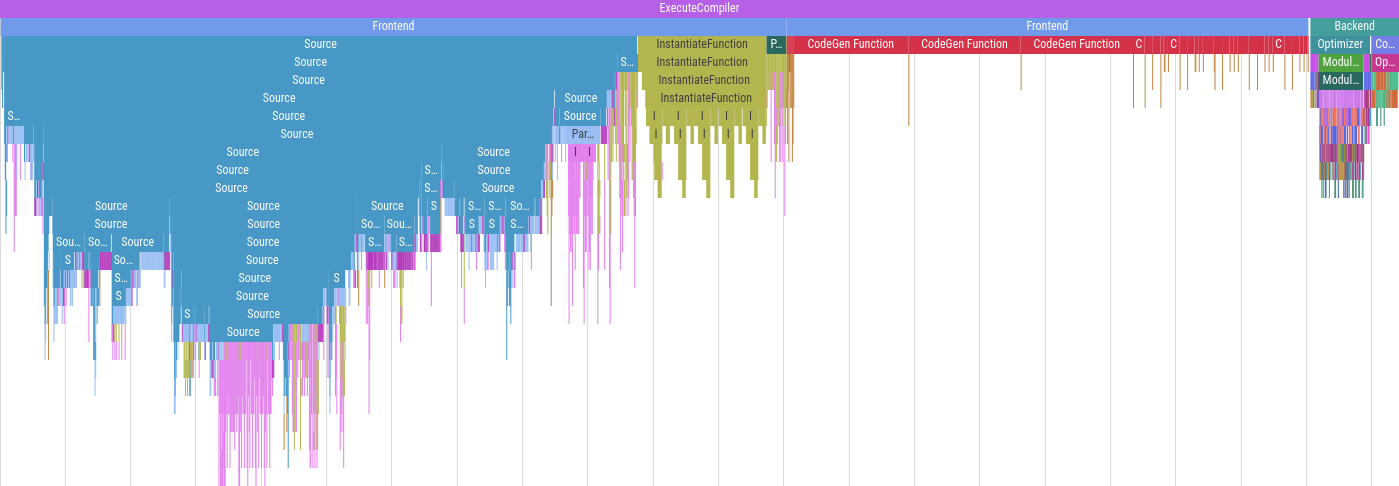
\includegraphics[scale=0.425, angle=90]{images/perfetto-ui.png}
\caption{Clang time trace file in Perfetto UI}
\label{fig:perfetto-time-trace-ui}
\clearpage
\end{figure}

The JSON files have a rather simple structure. They contain a
\lstinline{traceEvents} field that holds an array of JSON objects, each one of
them containing a \lstinline{name}, a \lstinline{dur} (duration), and
\lstinline{ts} (timestamp) field. It may also contain additional data in the
field located at \lstinline{/args/data}, as seen in listing
\ref{lst:clang-time-trace-event}. Duration and timestamps are expressed in
microseconds.

\begin{lstlisting}[
  language=json,
  caption=Time trace event generated by Clang's internal profiler,
  label=lst:clang-time-trace-event]{}
{
  "pid": 8696,
  "tid": 8696,
  "ph": "X",
  "ts": 3238,
  "dur": 7,
  "name": "Source",
  "args": {
    "detail": "/usr/include/bits/wordsize.h"
  }
}
\end{lstlisting}

In this example the \lstinline{/args/detail} field indicates the file that's
being processed durin this trace event. This field may also contain details
related to symbols being processed for events like
\lstinline{InstantiateFunction}.

Clang's profiling data is both very exhaustive as it covers
all compilation stages, but also very insightful as every timer event is
annotated with metadata that relates to specific \cpp symbols.
It can be extracted automatically by adding a compilation flag,
and there is a multitude of libraries that can parse its JSON output.

As such, the choice was made to reuse this data by making a tool to help
automate the extraction, analysis, and comparison of time trace files
for variable size compile time benchmarking.

\end{document}
